%================================================================================
%=============================== DOCUMENT SETUP =================================
%================================================================================

\documentclass[lang=english,inputenc=utf8,fontsize=10pt]{ldvarticle}
%PACKAGES

\usepackage{parskip}
\usepackage{subfigure}
\usepackage{ifthen}
\usepackage{comment}
\usepackage{color}
\usepackage{colortbl}
\usepackage{soul}
\usepackage{tikz}
\usetikzlibrary{shapes,arrows}
\usepackage{tabularx}
\usepackage{lipsum}
\definecolor{lightgray}{rgb}{0.75,0.75,0.75}
\usepackage{enumitem}
\setlistdepth{9}
%Image-related packages
\usepackage{graphicx}
\usepackage{float}
% \graphicspath{{./img/}
\usepackage{subcaption}
\usepackage[export]{adjustbox}
\usepackage{wrapfig}
\usepackage{blindtext}
\usepackage{array}
\usepackage{multirow}
\usepackage{appendix}
\setcitestyle{square}
%================================================================================
%================================= TITLE PAGE ===================================
%================================================================================

\title{The Greatest Work of Art }
\subtitle{Project report}
\author{Yan Gao\\
03750215
\and
Chenghao Hu\\
03743184
\and
Xue Zhang\\
03740499
\and
Yiming Shan\\
03749627  
\and
Ziyou Tang\\
03756512
\and
Zheng Tao\\
03740066
\and
Chi Wang\\
03736626
\and
Jinghan Zhang\\
03750520
\and
Kaicheng Ni\\
03749628
}

\date{\today}

\begin{document}


\maketitle
\thispagestyle{empty}

\hrule

\section*{Motivation}
Nowadays, the prosperous automobile industries has a close relationship with the increasing number of car incidents. The car rental companies are facing the problem of how to detect car damages faster and more precisely so that they can provide the insurance company accurate and real-time information. Given the dataset provided by \textit{WENN}, our project is aimed at classifying possible damages on cars by machine learning and deep learning-based algorithms. We would like to provide an easy-to-use and reliable method to fulfill this goal. To improve our accuracy, we will do dataset enrichment, data preprocessing, classification model comparison. We also want our model to keep updating after deployment, so we introduce Continual Learning method. We will also provide a website for user, which is not included in this report.
\vspace*{1cm}
\hrule

\newpage
\tableofcontents

\newpage
\section{Project Description}

Given a dataset containing images with all different types of damage, we want to build a classification model that can distinguish between them. However, the challenge we face is that only a limited number of labeled images are provided, while most other images are unlabeled, which means that our algorithm should be trained as efficiently as possible to keep the number of required labels low. During this period, we need not only to process the already labeled images to make them suitable for the classification task but also to enrich the dataset to meet the huge demand for labeled images during the training process.

\subsection{Research Question}
\begin{enumerate}
\item What machine learning algorithms can help us overcome the problem of lack of labeled datasets?
\item What kinds of machine learning algorithms help us to correct false labeled images in real time?
\item Does the resolution affect the accuracy of the classification?
\end{enumerate}



\subsection{Goals}
We have divided our project into several parts. The first part is the data preprocessing part, where we want to make the images suitable for our task. The second part is the base classification model part, where we plan to select several effective classification models. The third part is the dataset enrichment part, where we want to get more labeled images by some machine learning algorithms or even manually. The fourth part is the continuous learning part, where we aim to make our model "greedy" to acquire new knowledge, which means it can learn from new images and maintain its performance. The last part is the visualization part, where we want to show all our efforts on the website and make the interactions run smoothly.


\newpage

\section{Data basis}
By analyzing the given dataset, we found that there are more than 50K images in the whole dataset, while only 731 images are labeled. Among these labeled images, we obtained several key messages. First, all these damages are too difficult to locate. Second, most of the damage was limited by the shooting conditions and could not be accurately identified with the naked eye. Third, the rims were always the easiest to identify because the features were the most obvious. Fourth, the dent category and the other category are always easy to be confused.


\subsection{Sources}
We used the dataset provided by \textit{WENN} and relied mainly on labeled images. In addition, we manually labeled 230 images according to the given taxonomy.

\subsection{Data collection}
For a given raw image, its form is far from the way we can use it. We first need to change its format from .wepb to .jpeg. Secondly, we need to read and understand the given .json file. It contains a lot of information, and we need to extract useful information. For an annotated image, we find that the most useful information is the coordinates of the bounding box and the label of the image. With the bounding box, we can crop the corresponding image, so that the task becomes a classification task. With the labels, we can build a dataset based on these images and labels for training and testing. A problem here is that the resolution of images in different categories is quite different. For example, the size of an image labeled as a dent is several times smaller than the size of an image labeled as a rim. Therefore, we need to unify the size of the images, which is a prerequisite for the CNN input, with a uniform size of 224x224. In the last step, we need to classify all the labeled enlarged images according to their labels. Finally, we obtain a dataset with four categories: dent, rim, scratch, and other, which contains 272 images of dent, 220 images of rim, 193 images of scratch, and 46 images of other.\\

The datasets are a little bit hard to classify, even for human eyes. There are some images that contain more than one type of defect in the same area, but with only one bounding box. In this case, we labeled this type of image with two corresponding labels. Some images, like scratch and dent, are existed in the same area. Different people may come out with different labels for one class. In this situation, we labeled the data by three people so that we can avoid some mistakes. Labelers must be extremely focused because each error or inaccuracy negatively affects a dataset’s quality and the overall performance of a predictive model.\\

Some new data have been collected in addition to the known data set. There are 110 new data: 20 images of the scratch, 50 images of the rim, 20 images of the dent, and 20  images of others. When collecting the data, images of different sizes and resolutions have been selected to make the data more diverse. These additional data can be tested for the robustness of the model on different data sets.\\


\subsection{Preprocessing}
The first step we did for the preprocessing is to resize the input images with different sizes into the required input size of our two networks ResNet18 and VGG16, namely 224x224. This step is done by the PyTorch transform.Resize() command, which has changed the resolution of the original input images. One of our assumptions is that the resolution of the resized images could also lead to wrong answers of classification. Therefore we came to the idea of enlarging the size of the enlarged data before we fed the images into the standard resize process. To be more specific, for the given bounding boxes with sizes smaller than 224x224, namely the ones has to be interpolated during the resize process, we enlarged a larger bounding box of size 224x224 instead of the original ones so that the resolution of these images will not be worse in the later steps. To investigate the effect of this idea the training process is divided into two cases, namely: before enlarging and after enlarging.\\

In addition to resizing, we normalize the inputs as well. Because the networks we used are pretrained networks, which means they are already trained on some datasets, like ImageNet. Considering that ImageNet contains 20,000 categories and our dataset has a more sophisticated focus on one sub-category of the category “car” and the different parameters(mean and standard deviation) from two datasets may lead to different results we applied two pairs of parameters of normalization to our dataset for normalization: one pair of mean and standard deviation from ImageNet, the other from our own dataset.\\

Another challenge is the scarcity and insufficient variability of the dataset, the original dataset we obtained contains about 730 images which is not enough to achieve a high classification accuracy. Therefore we applied augmentation on the dataset with the help of the augmentation operations in Pytorch, which includes the basic augmentation operations like Grayscale, HorzontalFlip, and the sophisticated combination of some basic operations offered by Pytorch build-in functions like AugMix(). For comparison, we also apply non-augmentation and random combinations of basic ones. The build-in AugMix combines the basic operations in a stochastic way and solves the problem of unexpected augmentation results at the same time by mixing together the results of several augmentation chains in convex combinations and applying the consistency loss, for which we may expect a better result in the training.\\

During the training we tried all the possible combinations of preprocessing mentioned above: 
\begin{enumerate}
    \item enlarged data or non-enlarged data
    \item new or original normalization parameter
\end{enumerate}

After going through the two above steps we applied all augmentation we choose to the data, for instance, we train a ResNet on into 224x224 enlarged data which goes through different augmentation respectively and is normalized with the mean and standard of ImageNet. Then we compare the training and test results in this case for different augmentations. At last, we save the one with the best accuracy.


\newpage

\section{Data Model}
\subsection{Basic Models}
Here we provide the basic models we used in this project. The dummy model is only trained in supervised way, while VGG and ResNet are trained in supervised, semi-supervised and active learning way, which will be discussed in section 3.2.
\subsubsection{Dummy Model}
The dummy model, which is the baseline of this project, is a "silly" model with very low accuracy. The Sift and K-means algorithms are used here. The Sift algorithm is used to calculate the feature values of the images, and then the K-means algorithm is used to cluster the images. The existing dataset has been trained and divided into four categories: scratch, rim, dent, and other damage.

\subsubsection{ResNet and VGG}
VGG and ResNet models are functional convolutional deep neural networks in the computer vision field, therefore, we use the transfer learning technique of them to train our model. By loading a pre-trained model and resetting the final fully connected layer into four different classes (scratch, rim, dent, and other), we can easily achieve the damage classification task here. Considering network complexity and computation efficiency, ResNet18 and VGG16 networks are used in our project. 



\subsection{Approach}
As we mentioned before, we only have a limited dataset. But a good classification neural network always needs a large dataset. For example, we always retrain a pretraind PyTorch model to obtain better performance. This kind of pretrained PyTorch model is trained on the ImageNet dataset which contains nearly 15 million images. By doing research, we find that active learning can help us to resolve this problem.

\subsubsection{Active Learning}
Active learning is a field of machine learning that reduces labeling cost by only labeling the most informative examples. Datasets, especially in industry, contain many similar examples that would bring no information to the model.\\

To select the next example to label, we first train a machine learning model on the trained dataset. Then we compute the model’s uncertainty on all unlabeled examples. The most uncertain is selected to be labeled.\\

In this project, we implemented an active learning algorithm based on the Baal framework. It provides us with the basis for Bayesian active learning, by framing the problem from a Bayesian perspective. From our side, the most important part is the estimation of uncertainty. We use MC-Dropout to sample from the posterior distribution, allowing us to better estimate uncertainty. \\

\subsubsection{Semi-supervised Learning}
There is another automatic method to solve the problem with a small amount of labeled data and a large amount of unlabeled data, which is called Semi-Supervised Learning(SSL). SSL is a method between unsupervised learning and supervised learning\cite{ref2}.\\

There are various ways to realize SSL, like self-training. Self-training uses a small amount of labeled data to train an original model, then it generates pseudo labels from some unlabeled data and retrains with pseudo labeled data. However, this method tends to lead the model toward a biased direction.\\

The semi-supervised learning method we accepted is called SimCLR: A simple framework for contrastive learning of visual representations. It first uses unsupervised contrastive learning which takes two augmented versions of unlabeled images and lets the ResNet model learn the similarity between them. This ResNet takes an image as input and outputs a representation of it. A learnable nonlinear transformation between the representation and the contrastive loss substantially improves the quality of the learned representations. Next, it takes traditional supervised learning to train the ResNet with a small amount of labeled images.\\

The benefit of semi-supervised learning is that it does not require human labeling during the training process and the state-of-the-art method like SimCLR proposed by 
Geoffrey Hinton in 2020 very good performance in ImageNet. Although now there exist butter semi-supervised learning methods, we still choose SimCLR because it is easy to find PyTorch examples and tips online.

\subsubsection{Continual Learning}
The first two machine learning solutions addressed the pain point of insufficient datasets. Now, we wanted to find an algorithm that would give our classification neural network the ability to correct these mislabeled samples.\\

Through our research, we found that continuous learning provides a way to not only allow neural networks to gain new knowledge from new samples, but also to keep the knowledge they have learned so far.\\

In our project, we implemented algorithms for continuous learning on top of the Avalanche library. It provides dozens of continuous learning strategies and we implemented several of them and tested them on our complementary dataset.\\


\subsection{Training}
\subsubsection{Supervised Learning of Resnet and VGG}
% As have already discussed how to collect label data from the upper chapter, 
The Simplest way to train the networks is the supervised learning. Since the dataset is not too large and we have already labeled them all, we can study ResNet18 and VGG16 to get an impression of the performance we can achieve by further study. Firstly, we split the dataset into training and validation in the ratio of 80:20. Then we implement a preprocessing pipeline, which discussed before. Then we set the optimization function as SGD and loss function as CrossEntropyLoss to guide our model training processing. During each training epoch, the training and validation curve is shown in real time. The model parameters among all the epochs with the best validation performance will be saved.\\

\begin{figure}[h!]
    \centering
    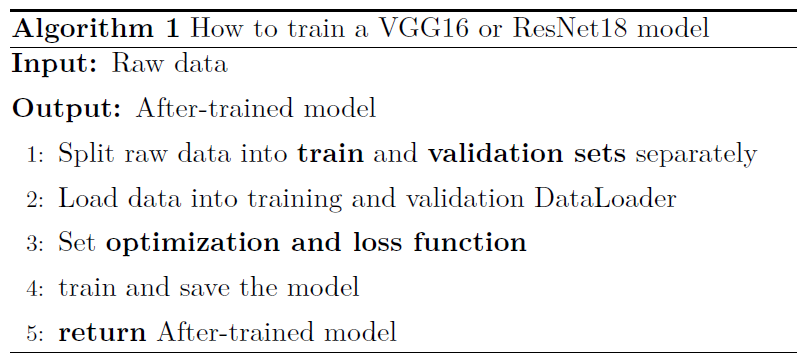
\includegraphics[scale=0.5]{train_VGG_ResNet18.png}
    % \caption{Different Foot Type}
    % \label{fig:feet}
\end{figure}

\subsubsection{Active Learning of VGG}
Due to the limited dataset, we made a slight change to our training procedure. We split our supplementary dataset into training and validation datasets and assume that the labels in the dataset do not exist. Our initial model is the ImageNet pretrained model and we change the number of classification into 4.\\
First, our model randomly selects 10 samples from the training dataset and manually labels them. Then, we train our model on these labeled images. After that, our model successively selects the first 10 uncertain samples and labels them. After that, we retrain these labeled samples. This process stops when the training accuracy reaches a certain threshold or the entire training dataset has been completely traversed.\\
% \begin{center}
%     \textcolor{red}{Algorithm}\\
% \end{center}

% \begin{figure}[h]
%     \centering
%     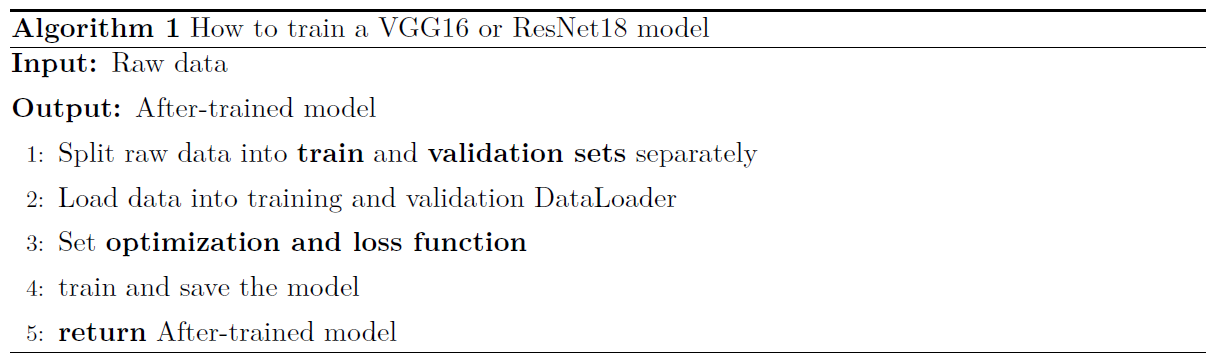
\includegraphics[scale=0.3]{VGG16andResNet18.png}
%     % \caption{Different Foot Type}
%     % \label{fig:feet}
% \end{figure}

% \begin{figure}[h!]
%     \centering
%     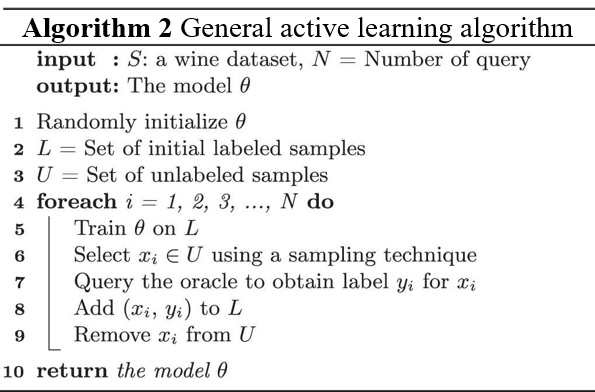
\includegraphics[scale=1]{active learning.png}
%     % \caption{Different Foot Type}
%     % \label{fig:feet}
% \end{figure}

\subsubsection{Semi-Supervised Learning of Resnet}
Unlike self-training, SimCLR is first trained with unlabeled data, then with labeled data. The first step is fulfilled with a method called contrastive learning. Two separate data augmentation operators are applied to each data example to obtain two correlated views. A base encoder network f(·) and a projection head g(·) are trained to maximize agreement using a contrastive loss. After training, we throw away the projection head g(·) and use encoder f(·) and representation h for downstream tasks.
\begin{figure}[h]
    \centering
    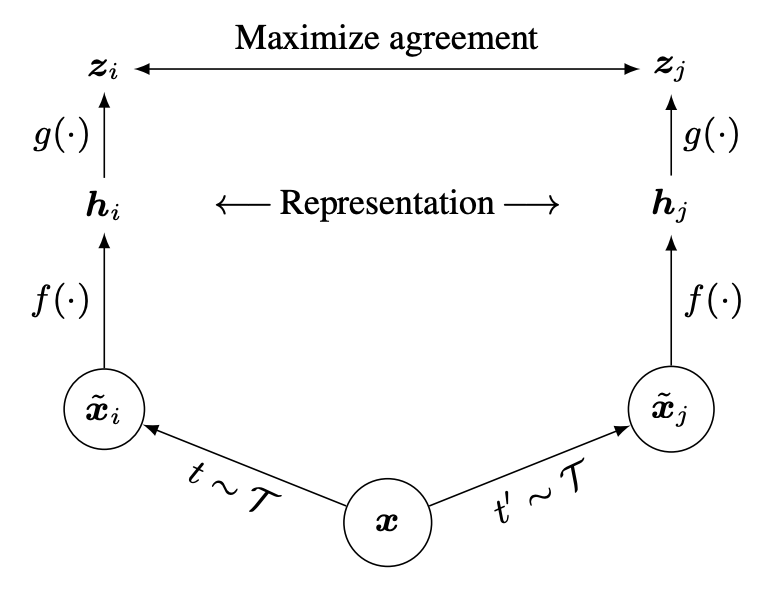
\includegraphics[scale=0.3]{Semi.png}
    \caption{Contrastive Learning Structure}
    \label{Semi structure}
\end{figure}

\subsubsection{Continual Learning to Retrain}
After we picked out these samples with uncorrected labels and manually labeled them. We trigger our continuous learning. We transfer the dataset to the stream and feed it to our continuous learning model. At the end of the whole training process, we get our new model.\\

In our project, we implement several strategies. The first one is the cumulative training strategy. In each experience, the model is trained with data from all previous experiences and current experiences. This strategy avoids catastrophic forgetting because it trains all the experiences collected so far. We do not recommend this strategy because it consumes a lot of time and computational resources when the dataset is too large.\\

The second one is the Replay training strategy. This strategy relies mainly on common knowledge: it is widely believed that replaying past experiences can reduce the brain's forgetting. That is, a single learning network is fed with experiences (both new and replayed).\\

The third is the learning without forgetting (LWF) training strategy. This strategy makes clever use of knowledge distillation techniques. Specifically, the old model is used as a teacher model for each sample in the new task.\\

The last type is the Naive training model. This is the simplest (and least effective) continuous learning strategy. naive only incrementally fine-tunes a model and does not employ any method to compare the catastrophic forgetting of previous knowledge.\\

We will evaluate these four models on a complementary dataset and compare the results between them.\\


\subsection{Evaluation}
The evaluation indicators we accepted are accuracy, class-level precision rate, and class-level recall rate.\\

Accuracy is the number of correct predictions divided by the total number of predictions made. Accuracy is intuitive, but it doesn’t count how many True classes are misclassified as Negative and how many False classes are misclassified as Positive. In our multiclass case, the formula of Accuracy looks like this:

\begin{center}
    $Accuracy=\frac{TP+TN}{TP+TN+FP+FN}$
\end{center}
Class-level precision rate is slightly different from binary classification one. If there are four classes A, B, C, and D, the class-level precision is (Correctly predicted A)/(A predicted as A + B predicted as A + C predicted as A + D predicted as A)\\

Class-level recall rate is also different from binary one. If there are four classes A, B, C, and D, the class-level precision is (Correctly predicted A)/(A predicted as A+A\\ predicted as B+... + A predicted as D)

We did not accept class-level F1-Score because this may not be intuitive for a user without a data analysis background.




\newpage

\section{Results}
So far, we have presented all the models used in our project and the strategies to evaluate their performance. In the following section, we will analyze these results in depth and give our observations and further analysis.\\
For the result we consider the training, validation loss, validation accuracy, and the recall and precision for each category during the test. 

\subsection{Observations}

\subsubsection{Prediction of Dummy model}
Figure \ref{dummy} is a result of the dummy model, which can be seen is that the input image is actually a rim, but after the dummy model, the detected result is scratch, and the score is 0.525. This result is wrong and the dummy model is very "stupid". Therefore, in the following analysis we will not compare other models with it.\\

% \begin{center}
%     \textcolor{red}{Figure}\\
% \end{center}
\begin{figure}[H]
    \centering
    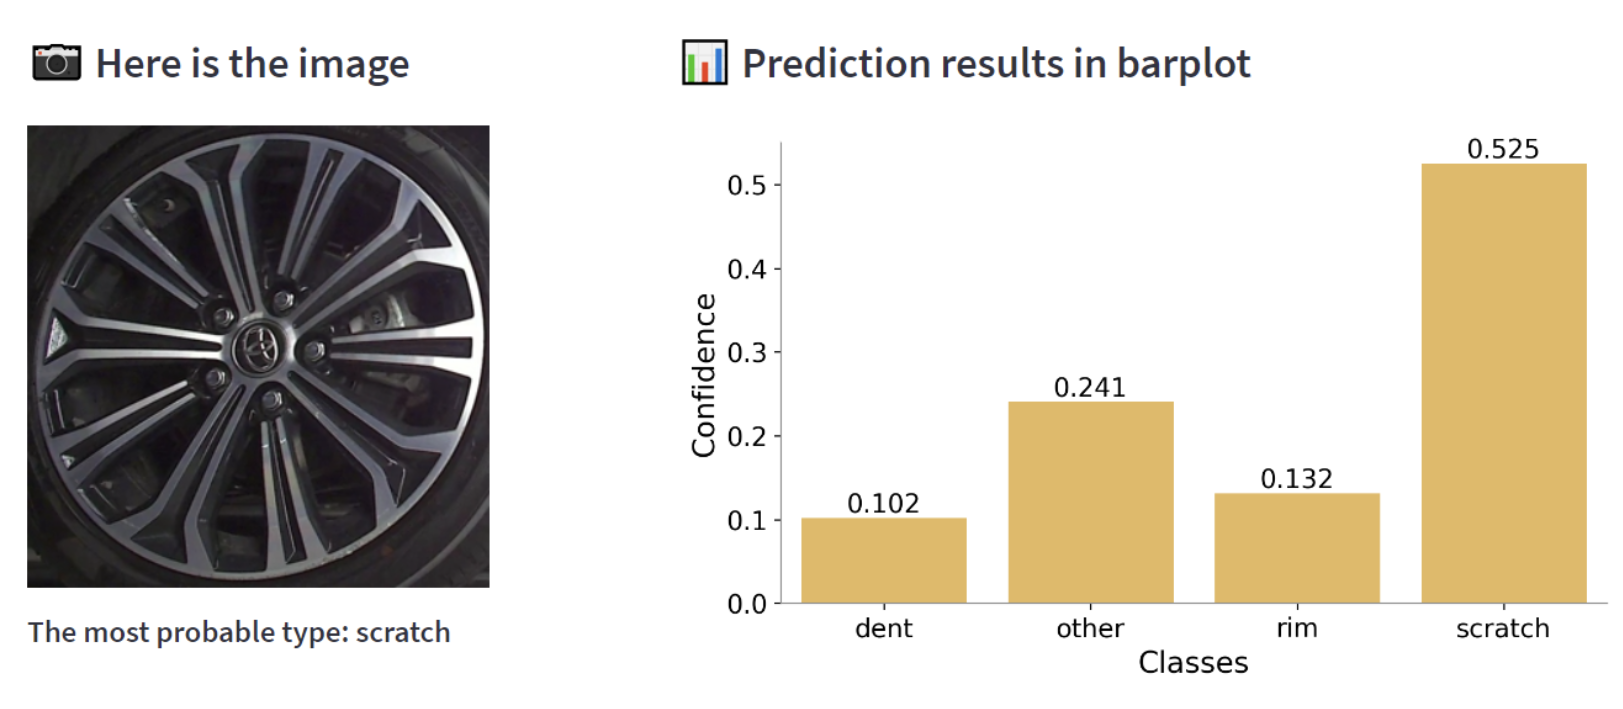
\includegraphics[scale=0.2]{resultDummy.png}
    \caption{The Result of dummy model}
    \label{dummy}
\end{figure}

\subsubsection{Performance of ResNet and VGG}
\begin{enumerate}[label=\alph*)]
    \item 
    The ResNet with the best performance(Acc) we can achieve is shown in table \ref{Preprocessing and Hyperparameters for best Resnet}. We chose the preprocessing pipeline and Hyper-parameters as follows:\\
    \begin{table}[H] 
        \begin{center}  
            \caption{Preprocessing and Hyper-parameters for best Resnet}  
            \label{Preprocessing and Hyperparameters for best Resnet}
            \begin{tabular}{|m{2cm}<{\centering}|m{2cm}<{\centering}|m{2cm}<{\centering}|m{2cm}<{\centering}|m{2cm}<{\centering}|m{2cm}<{\centering}|}   
            \hline   \textbf{Transform} & \textbf{Learning rate}& \textbf{Batch Size} & \textbf{Loss Function} & \textbf{Enlarged} & \textbf{Acc(\%)} \\   
            \hline   Horizontal Flip & 0.0010 & 4 & cross entropy & False & 92.57 \\  
            \hline   
            \end{tabular}   
        \end{center}  
    \end{table}
    \begin{table}[H]   
        \begin{center}   
        \caption{Class-Level Result of the Best ResNet}  
        \label{ResNet performance} 
        \begin{tabular}{|m{2cm}<{\centering}|m{2cm}<{\centering}|m{2.0cm}<{\centering}|m{2cm}<{\centering}|m{2cm}<{\centering}|}   
        \hline   &\textbf{dent} & \textbf{scratch} & \textbf{other} & \textbf{rim}\\ 
        % \hline   \textbf{precision rate}  & 0.910714 & 0.918919 & 0.727273 & 1.000000  \\ 
        % \hline   \textbf{recall rate} & 0.927273 & 0.871795 & 0.8 & 1   \\
        \hline   \textbf{precision rate}  & 0.9107 & 0.9189 & 0.7272 & 1.0000  \\ 
        \hline   \textbf{recall rate} & 0.9272 & 0.8717 & 0.8000 & 1.0000   \\
        \hline 
        \end{tabular}   
        \end{center}   
    \end{table}
    \item
    The VGG with the best performance(Acc) we can achieve is shown in table \ref{Preprocessing and Hyperparameters for best VGG}. We chose the preprocessing pipeline and Hyper-parameters as follows:\\
    \begin{table}[H] 
        \begin{center}  
            \caption{Preprocessing and Hyper-parameters for best VGG}  
            \label{Preprocessing and Hyperparameters for best VGG}
            \begin{tabular}{|m{2cm}<{\centering}|m{2cm}<{\centering}|m{2cm}<{\centering}|m{2cm}<{\centering}|m{2cm}<{\centering}|m{2cm}<{\centering}|}   
            \hline   \textbf{Transform} & \textbf{Learning rate}& \textbf{Batch Size} & \textbf{Loss Function} & \textbf{Enlarged} & \textbf{Acc(\%)} \\   
            \hline   Vertical Flip & 0.0001 & 16 & cross entropy & False & 93.92 \\  
            \hline   
            \end{tabular}   
        \end{center}  
    \end{table}
        \begin{table}[htb]   
        \begin{center}   
        \caption{Class-Level Result of the Best VGG}  
        \label{VGG performance} 
        \begin{tabular}{|m{2cm}<{\centering}|m{2cm}<{\centering}|m{2.0cm}<{\centering}|m{2cm}<{\centering}|m{2cm}<{\centering}|}   
        \hline   &\textbf{dent} & \textbf{scratch} & \textbf{other} & \textbf{rim}\\ 
        \hline   \textbf{precision rate}  & 0.9455 & 0.8750 & 0.8889 & 1.0000  \\ 
        \hline   \textbf{recall rate} & 0.9455 & 0.8974 & 0.8000 & 1.0000   \\  
        \hline 
        \end{tabular}   
        \end{center}   
    \end{table}
\end{enumerate}



% After training, we obtained eight different tables like table \ref{table resnet crop} above for our comparison.
% In terms of enlarging, we first compared the accuracy of the Resnet trained on data normalized with mean and standard deviation on the ImageNet. The one before enlarging has an average accuracy of 0.8806 the one with enlarging 0.8817, from which it is hard to tell the influence of the enlarging. Taking a closer look at the result we found that the one without enlarging achieved about 0.02 improvement when some augmentation was applied to the dataset(left), while for the enlarged data(right) a second highest accuracy was already achieved for non -transformation and there is not much difference between this one and the one with the highest accuracy.

% \begin{table}[h] 
% \begin{center}  
% \caption{Performance of enlarging for Resnet}  
% % \label{table:1} 
% \label{table resnet crop}
% \begin{tabular}{|m{2.4cm}<{\centering}|m{6cm}<{\centering}|m{2.0cm}<{\centering}|}   
% \hline   \textbf{Transform} & \textbf{Description} & \textbf{acc} \\   
% \hline   0 & no transform(except resize and normalize) & 0.898649  \\  
% \hline   6Invert & common single basic transform & 0.912162  \\      
% \hline   
% \end{tabular}   
% \end{center}  
% \end{table}

% \begin{table}[htb]   
% \begin{center}   
% \caption{Performance of enlarging for Resnet}  
% \label{table VGG crop} 
% \begin{tabular}{|m{2.4cm}<{\centering}|m{6cm}<{\centering}|m{2.0cm}<{\centering}|}   
% \hline   \textbf{Transform} & \textbf{Description} & \textbf{acc} \\  
% \hline   0 & no transform(except resize and normalize) & 0.912162  \\  
% \hline   6HorizontalFlip & common single basic transform & 0.918919  \\      
% \hline   
% \end{tabular}   
% \end{center}   
% \end{table}

% The same happened when we compared the results from the Resnet which trained on data with normalization parameters from our dataset with different enlarging operations. The similar results go for the VGG for the case with the normalization parameter of our data as well or even more obvious, where the highest accuracy of 0.93 is achieved for non-enlarged data by the augmentation random vertical flip while the highest accuracy for enlarged data is found in the case without augmentation(0.89).

% We also investigated the influence of the normalization parameter. The following table shows the average accuracy obtained by different preprocessing steps.


Among all the preprocessing possibilities we chose the Resnet and the VGG with the best accuracy, their training loss and validation loss plot are shown below, they are both trained on non-enlarged data which is normalized with the original mean and standard deviation. The augmentation used are horizontal flip and vertical flip.\\

From table\ref{Preprocessing and Hyperparameters for best Resnet}and table \ref{Preprocessing and Hyperparameters for best VGG} we see that the best accuracy of 0.925676 and 0.939189 are achieved for Resnet18 and VGG16 respectively.


\subsubsection{Performance of Active Learning}
In the training process, we adopt the Monte-Carlo Dropout and CrossEntropyLoss as criterion and SGD as optimizer, where learning rate is 0.001, momentum is 0.9 and weight\_decay is 0.0005.\\

The performance is firstly performed on validation set and then on the supplement dataset. And we compare the performance of Active learning model and VGG16 model on the same dataset. It is shown in table \ref{Active V} \textasciitilde \ref{VGG16 s} 

\begin{table}[H]   
    \begin{center}   
    \caption{Result of Active Learning on Validation dataset}  
    \label{Active V} 
    \begin{tabular}{|m{2cm}<{\centering}|m{2cm}<{\centering}|m{2.0cm}<{\centering}|m{2cm}<{\centering}|m{2cm}<{\centering}|}   
    \hline   &\textbf{dent} & \textbf{scratch} & \textbf{other} & \textbf{rim}\\ 
    \hline   \textbf{precision rate}  & 0.9019 & 0.7292 & 1.0000 & 1.0000  \\ 
    \hline   \textbf{recall rate} & 0.8364 & 0.8974 & 0.7000 & 0.9545   \\  
    \hline   \textbf{total accuracy(\%)} & \multicolumn{4}{|c|}{87.83} \\  
    \hline 
    \end{tabular}   
    \end{center}   
\end{table}

\begin{table}[H]   
    \begin{center}   
    \caption{Result of VGG16 on Validation dataset}  
    \label{VGG16 V} 
    \begin{tabular}{|m{2cm}<{\centering}|m{2cm}<{\centering}|m{2.0cm}<{\centering}|m{2cm}<{\centering}|m{2cm}<{\centering}|}   
    \hline   &\textbf{dent} & \textbf{scratch} & \textbf{other} & \textbf{rim}\\ 
    \hline   \textbf{precision rate}  & 0.7777 & 0.6923 & 0.4000 & 0.9545  \\ 
    \hline   \textbf{recall rate} & 0.5091 & 0.6923 & 0.4000 & 0.9545   \\  
    \hline   \textbf{total accuracy(\%)} & \multicolumn{4}{|c|}{68.24} \\  
    \hline 
    \end{tabular}   
    \end{center}   
\end{table}

\begin{table}[H]   
    \begin{center}   
    \caption{Result of Active Learning on Supplement dataset}  
    \label{Active s} 
    \begin{tabular}{|m{2cm}<{\centering}|m{2cm}<{\centering}|m{2.0cm}<{\centering}|m{2cm}<{\centering}|m{2cm}<{\centering}|}   
    \hline   &\textbf{dent} & \textbf{scratch} & \textbf{other} & \textbf{rim}\\ 
    \hline   \textbf{precision rate}  & 0.2000 & 0.5000 & 0.4000 & 1.0000  \\ 
    \hline   \textbf{recall rate} & 0.2000 & 0.4000 & 0.6000 & 0.9000   \\  
    \hline   \textbf{total accuracy(\%)} & \multicolumn{4}{|c|}{60.00} \\  
    \hline 
    \end{tabular}   
    \end{center}   
\end{table}

\begin{table}[H]   
    \begin{center}   
    \caption{Result of VGG16 on Supplement dataset}  
    \label{VGG16 s} 
    \begin{tabular}{|m{2cm}<{\centering}|m{2cm}<{\centering}|m{2.0cm}<{\centering}|m{2cm}<{\centering}|m{2cm}<{\centering}|}   
    \hline   &\textbf{dent} & \textbf{scratch} & \textbf{other} & \textbf{rim}\\ 
    \hline   \textbf{precision rate}  & 0.3750 & 0.3330 & 1.0000 & 1.0000  \\ 
    \hline   \textbf{recall rate} & 0.6000 & 0.4000 & 0.2000 & 1.0000   \\  
    \hline   \textbf{total accuracy(\%)} & \multicolumn{4}{|c|}{64.00} \\  
    \hline 
    \end{tabular}   
    \end{center}   
\end{table}


\subsubsection{Performance of Semi-Supervised Learning}
The performance of Semi-Supervised Learning is also performed on validation set. It is shown in table \ref{semi performance}. \\
\begin{table}[ht]   
    \begin{center}   
    \caption{Result of Semi-Supervised Learning}  
    \label{semi performance} 
    \begin{tabular}{|m{2cm}<{\centering}|m{2cm}<{\centering}|m{2.0cm}<{\centering}|m{2cm}<{\centering}|m{2cm}<{\centering}|}   
    \hline   &\textbf{dent} & \textbf{scratch} & \textbf{other} & \textbf{rim}\\ 
    \hline   \textbf{precision rate}  & 0.7582 & 0.5730 & 0.8571 & 0.9639  \\ 
    \hline   \textbf{recall rate} & 0.7113 & 0.6986 & 0.3333 & 0.9756   \\  
    \hline   \textbf{total accuracy(\%)} & \multicolumn{4}{|c|}{76.30} \\  
    \hline 
    \end{tabular}   
    \end{center}   
\end{table}

\subsubsection{Performance Continual Learning}
For evaluation, we consider the training and validation accuracy, training, and validation loss.  We mainly compare the performance of two continual learning strategies: cumulative training strategy and learning without forgetting (LWF) training strategy. \\

Cumulative training strategy:
In the training process, we adopt CrossEntropyLoss as a criterion and SGD as an optimizer, where the learning rate is 0.0010 and the momentum is 0.9.\\

LWF training strategy: In the training process, we adopt CrossEntropyLoss as criterion and SGD as an optimizer, where the learning rate is 0.0010 and momentum is 0.9. Alpha is 1 and temperature is 2.\\

% \begin{figure}[h]
%     \centering
%     \begin{subfigure}{}
%     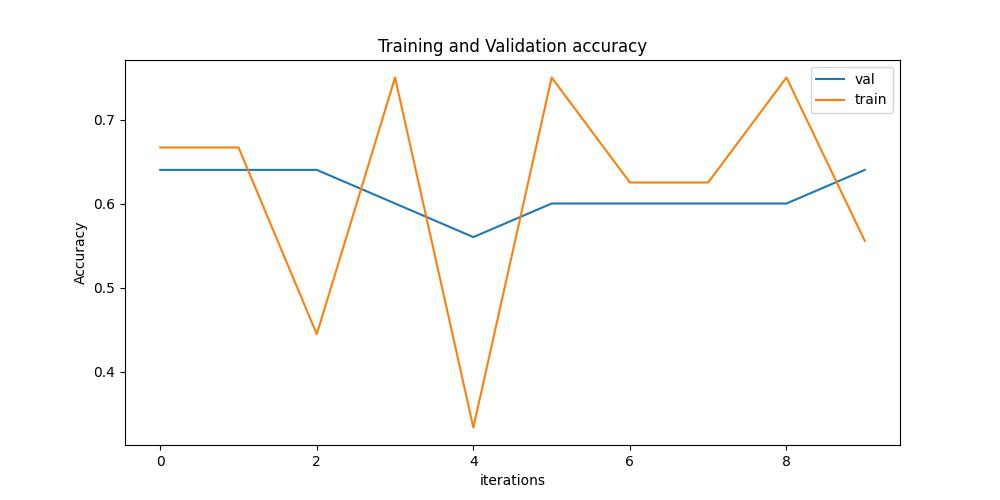
\includegraphics[scale=0.4]{conV11.png}
%     \end{subfigure}
%     \begin{subfigure}{}
%     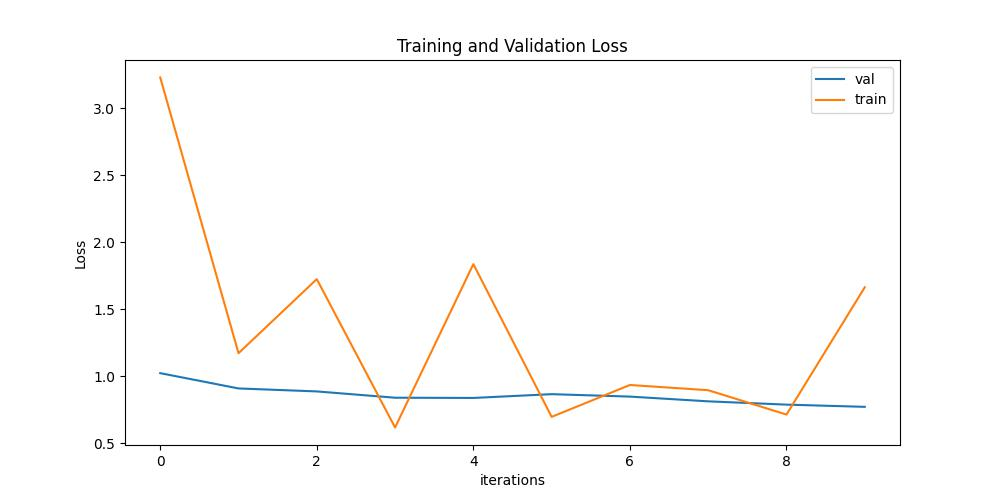
\includegraphics[scale=0.4]{conV22.png}
%     \end{subfigure}
%     \caption{VGG16's Training and validation accuracy and loss}
% \end{figure}






Our validation dataset is obtained from the supplement dataset.


\subsection{Trends}
    % \begin{enumerate}
    %     \item \textbf{Resnet and VGG}
            % \begin{table}[H]   
            %     \begin{center}   
            %     \caption{Result of ResNet18}  
            %     \label{Result of ResNet18} 
            %     \begin{tabular}{|m{2cm}<{\centering}|m{2cm}<{\centering}|m{2.0cm}<{\centering}|m{2cm}<{\centering}|m{2cm}<{\centering}|}   
            %     \hline   &\textbf{dent} & \textbf{scratch} & \textbf{other} & \textbf{rim}\\ 
            %     \hline   \textbf{precision rate}  & 0.925925926 & 0.85 & 1 & 0.936170213  \\ 
            %     \hline   \textbf{recall rate} & 0.909090909 & 0.871794872 & 0.7 & 1   \\  
            %     \hline   \textbf{total accuracy} & \multicolumn{4}{|c|}{0.912162162} \\  
            %     \hline 
            %     \end{tabular}   
            %     \end{center}   
            % \end{table}
    %         \begin{table}[htb]   
    %             \begin{center}   
    %             \caption{Result of VGG16}  
    %             \label{Result of VGG16} 
    %             \begin{tabular}{|m{2cm}<{\centering}|m{2cm}<{\centering}|m{2.0cm}<{\centering}|m{2cm}<{\centering}|m{2cm}<{\centering}|}   
    %             \hline   &\textbf{dent} & \textbf{scratch} & \textbf{other} & \textbf{rim}\\ 
    %             \hline   \textbf{precision rate} & 0.833334 & 0.72727273 & 1 & 0.95555556   \\  
    %             \hline   \textbf{recall rate}  & 0.81818182 & 0.82051282 & 0.5 & 0.97727273  \\ 
    %             \hline   \textbf{total accuracy} & \multicolumn{4}{|c|}{0.844594595} \\  
    %             \hline 
    %             \end{tabular}   
    %             \end{center}   
    %         \end{table}
    %     \item \textbf{Semi-Supervised Learning}
            
    %     \item \textbf{Active learning}
    %         \begin{enumerate}
    %             \item Do evaluation on the validation dataset obtained from original dataset
    %                 \begin{enumerate}
    %                     \item Active leanring model
    %                         \begin{enumerate}
    %                             \item class recall\_rate: {'dent':0.8363636363636363, 'scratch': 0.8974358974358975, 'other': 0.7, 'rim': 0.9545454545454546}
    %                             \item total acc: 0.8783783783783784
    %                             \item class precision\_rate:{'dent': 0.9019607843137255, 'scratch': 0.7291666666666666, 'other': 1.0, 'rim': 1.0}
    %                         \end{enumerate}
    %                     \item Well trained VGG16 model
    %                         \begin{enumerate}
    %                             \item class recall\_rate: {'dent': 0.509090909090909, 'scratch': 0.6923076923076923, 'other': 0.4, 'rim': 0.9545454545454546} 
    %                             \item total acc: 0.6824324324324325
    %                             \item class precision\_rate: {'dent': 0.7777777777777778, 'scratch': 0.4909090909090909, 'other': 0.4, 'rim': 0.8936170212765957}
    %                         \end{enumerate}
    %                 \end{enumerate}
    %             \item Do evaluation on the supplement dataset
    %                 \begin{enumerate}
    %                         \item Active leanring model
    %                             \begin{enumerate}
    %                                 \item class recall\_rate: {'dent': 0.2, 'scratch': 0.6, 'other': 0.4, 'rim': 0.9}
    %                                 \item total acc: 0.6
    %                                 \item class precision\_rate: {'dent': 0.2, 'scratch': 0.5, 'other': 0.4, 'rim': 1.0}
    %                             \end{enumerate}
    %                         \item Well trained VGG16 model
    %                             \begin{enumerate}
    %                                 \item class recall\_rate: {'dent': 0.6, 'scratch': 0.4, 'other': 0.2, 'rim': 1.0} 
    %                                 \item total acc: 0.64
    %                                 \item class precision\_rate: {'dent': 0.375, 'scratch': 0.3333333333333333, 'other': 1.0, 'rim': 1.0}
    %                             \end{enumerate}
    %                 \end{enumerate}
    %         \end{enumerate}
    %     \item \textbf{Continual learning}
    %         \begin{enumerate}
    %                 \item Comparison between the best vgg16 model and continual learning model on validation dataset obtained from supplement dataset
    %                     \begin{enumerate}
    %                         \item VGG16
    %                             \begin{enumerate}
    %                                 \item class recall\_rate: {'dent': 0.6, 'scratch': 0.4, 'other': 0.2, 'rim': 1.0} 
    %                                 \item total acc: 0.64
    %                                 \item class precision\_rate: {'dent': 0.375, 'scratch': 0.3333333333333333, 'other': 1.0, 'rim': 1.0}
    %                             \end{enumerate}
    %                         \item Cumulative training strategy
    %                             \begin{enumerate}
    %                                 \item class recall\_rate: {'dent': 0.0, 'scratch': 0.4, 'other': 0.6, 'rim': 1.0} 
    %                                 \item total acc: 0.6
    %                                 \item class precision\_rate: {'dent': 0.0, 'scratch': 0.3333333333333333, 'other': 0.42857142857142855, 'rim': 0.9090909090909091}
    %                             \end{enumerate}
    %                         \item learning without forgetting (LWF) training strategy
    %                             \begin{enumerate}
    %                                 \item class recall\_rate: {'dent': 0.2, 'scratch': 0.2, 'other': 0.8, 'rim': 1.0}
    %                                 \item total acc: 0.64
    %                                 \item class precision\_rate: {'dent': 0.3333333333333333, 'scratch' : 0.3333333333333333, 'other': 0.5714285714285714, 'rim': 0.8333333333333334}
    %                             \end{enumerate}
    %                     \end{enumerate}
    %                 \item Comparison between the best resnet18 model and continual learning model on validation dataset obtained from supplement dataset
    %                     \begin{enumerate}
    %                             \item ResNet18
    %                                 \begin{enumerate}
    %                                     \item class recall\_rate: {'dent': 0.4, 'scratch': 0.4, 'other': 0.0, 'rim': 0.8}
    %                                     \item total acc: 0.48
    %                                     \item class precision\_rate: {'dent': 0.2, 'scratch': 0.6666666666666666, 'other': 0.0, 'rim': 0.8888888888888888}
    %                                 \end{enumerate}
    %                             \item cumulative training strategy
    %                                 \begin{enumerate}
    %                                     \item class recall\_rate: {'dent': 0.4, 'scratch': 0.4, 'other': 0.0, 'rim': 0.9}  
    %                                     \item total acc: 0.52
    %                                     \item class precision\_rate: {'dent': 0.2222222222222222, 'scratch': 0.6666666666666666, 'other': 0.0, 'rim': 0.9}
    %                                 \end{enumerate}
    %                             \item learning without forgetting (LWF) training strategy
    %                                 \begin{enumerate}
    %                                     \item class recall\_rate: {'dent': 0.4, 'scratch': 0.2, 'other': 0.0, 'rim': 0.9} 
    %                                     \item total acc: 0.48
    %                                     \item class precision\_rate: {'dent': 0.2, 'scratch': 0.5, 'other': 0.0, 'rim': 0.9}
    %                                 \end{enumerate}
    %                     \end{enumerate}
    %             \end{enumerate}
    % \end{enumerate}
% \end{itemize}
Here we compare the results from the previous section and generalize our model on a supplement dataset.
\subsubsection{Resnet vs VGG}
    Here we compare the best VGG and the best ResNet we can get. And test their performance on supplement dataset. 
    \begin{table}[H]   
    \begin{center}   
    \caption{Best ResNet vs Best VGG}  
    \label{Resnet vs VGG} 
    \begin{tabular}{|m{2cm}<{\centering}|m{2cm}<{\centering}|m{2.0cm}<{\centering}|m{2cm}<{\centering}|m{2cm}<{\centering}|}   
    \hline   &\textbf{ResNet} & \textbf{VGG}\\ 
    \hline   \textbf{Acc(\%)}  & 92.57 & 93.92   \\ 
    \hline 
    \end{tabular}   
    \end{center}   
    \end{table}
    
    \begin{table}[H]   
    \begin{center}   
    \caption{Performance of ResNet and VGG on Supplementary Dataset}  
    \label{Resnet and VGG generalize} 
    \begin{tabular}{|m{2cm}<{\centering}|m{2cm}<{\centering}|m{2.0cm}<{\centering}|m{2cm}<{\centering}|m{2cm}<{\centering}|}   
    \hline   &\textbf{dent} & \textbf{scratch} & \textbf{other} & \textbf{rim}\\ 
    \hline   \textbf{ResNet precision rate}  & 0.3030  & 0.4103 & 0 & 1  \\ 
    \hline   \textbf{VGG precision rate}  & 0.4848 & 0.6087 & 1 & 0.9423 \\ 
    \hline   \textbf{ResNet recall rate} & 0.5000 & 0.8000 & 0 & 0.7600  \\  
    \hline   \textbf{VGG recall rate} & 0.8000  & 0.7000 & 0.1000 & 0.9800   \\  
    \hline   \textbf{Resnet total accuracy(\%)} & \multicolumn{4}{|c|}{58.18} \\  
    \hline   \textbf{VGG total accuracy(\%)} & \multicolumn{4}{|c|}{73.63} \\
    \hline 
    \end{tabular}   
    \end{center}   
\end{table}
\subsubsection{Enlarged vs Non-Enlarged}
    \begin{table}[H]   
    \begin{center}   
    \caption{ResNet enlarged vs non-enlarged}  
    \label{Resnet enlarge} 
    \begin{tabular}{|m{2cm}<{\centering}|m{2cm}<{\centering}|m{2.0cm}<{\centering}|m{2cm}<{\centering}|m{2cm}<{\centering}|}   
    \hline   &\textbf{enlargeded} & \textbf{non-enlarged}\\ 
    \hline   \textbf{Acc(\%)}  & 88.06 & 87.64   \\ 
    \hline 
    \end{tabular}   
    \end{center}   
    \end{table}
    
    \begin{table}[H]   
    \begin{center}   
    \caption{VGG enlarged vs non-enlarged}  
    \label{Resnet enlarge} 
    \begin{tabular}{|m{2cm}<{\centering}|m{2cm}<{\centering}|m{2.0cm}<{\centering}|m{2cm}<{\centering}|m{2cm}<{\centering}|}   
    \hline   &\textbf{enlargeded} & \textbf{non-enlarged}\\ 
    \hline   \textbf{Acc(\%)}  & 86.34 & 90.69  \\ 
    \hline 
    \end{tabular}   
    \end{center}   
    \end{table}
    

\subsubsection{Chosen of Normalization}
    \begin{table}[H]
    \begin{center}   
    \caption{Resnet ImageNet normalization vs Data-Based Normalization}  
    \label{Resnet normalization} 
    \begin{tabular}{|m{2cm}<{\centering}|m{2cm}<{\centering}|m{2.0cm}<{\centering}|m{2cm}<{\centering}|m{2cm}<{\centering}|}   
    \hline   &\textbf{ImageNet} & \textbf{Data-Based}\\ 
    \hline   \textbf{Acc(\%)}  & 88.06 & 87.49  \\ 
    \hline 
    \end{tabular}   
    \end{center}   
    \end{table}
    
    \begin{table}[H]
    \begin{center}   
    \caption{VGG ImageNet normalization vs Data-Based Normalization}  
    \label{Resnet normalization} 
    \begin{tabular}{|m{2cm}<{\centering}|m{2cm}<{\centering}|m{2.0cm}<{\centering}|m{2cm}<{\centering}|m{2cm}<{\centering}|}   
    \hline   &\textbf{ImagNet} & \textbf{Data-Based}\\ 
    \hline   \textbf{Acc(\%)}  & 86.34 & 85.30  \\ 
    \hline 
    \end{tabular}   
    \end{center}   
    \end{table}
    From the table, we notice that applying a pair of new normalization parameters from our own dataset does not help much to improve the accuracy.\\
\subsubsection{Active-Learning vs Semi-Supervised Learning}
The performance of active learning is better than semi-supervised learning in both validation set and supplementary set as shown in tabel \ref{Active vs Semi}
    \begin{table}[H]
    \begin{center}   
    \caption{Active Learning vs Semi-Supervised Learning}  
    \label{Active vs Semi} 
    \begin{tabular}{|m{2cm}<{\centering}|m{2cm}<{\centering}|m{2.0cm}<{\centering}|m{2cm}<{\centering}|m{2cm}<{\centering}|}   
    \hline   &\textbf{Active Learning} & \textbf{Semi-Supervised Learning}\\ 
    \hline   \textbf{Validation Accuracy(\%)}  & 87.84 & 76.30  \\ 
    \hline   \textbf{Generalization Accuracy(\%)}  & 60.00 & 56.36  \\ 
    \hline 
    \end{tabular}   
    \end{center}   
    \end{table}
\subsubsection{Continual Learning with Different Strategies}
    \begin{table}[H]
    \begin{center}   
    \caption{Comparison of Accuracy of Continual Learning Strategies}  
    \label{Continual compaer} 
    \begin{tabular}{|m{2cm}<{\centering}|m{2cm}<{\centering}|m{2.0cm}<{\centering}|m{2cm}<{\centering}|m{2cm}<{\centering}|}   
    \hline   Model&\textbf{Cumulative Training Strategy} & \textbf{LWF Training Strategy} & \textbf{Original Mode}\\ 
    \hline   \textbf{VGG16}  & 0.6000 & 0.6400 & 0.6400\\ 
    \hline   \textbf{Resnet}  & 0.5200 & 0.4800 & 0.4800\\ 
    \hline 
    \end{tabular}   
    \end{center}   
    \end{table}
    
    \begin{table}[h]   
    \begin{center}   
    \caption{Class-Level Comparison of Different Continual Learning Strategies}  
    \label{Class-Level Comparison CL} 
    \begin{tabular}{|m{2cm}<{\centering}|m{2cm}<{\centering}|m{2.0cm}<{\centering}|m{2cm}<{\centering}|m{2cm}<{\centering}|}   
    \hline   &\textbf{dent} & \textbf{scratch} & \textbf{other} & \textbf{rim}\\ 
    \hline   \textbf{CT precision rate(\%)}  & 0.7582 & 0.5730 & 0.8571 & 0.9639  \\ 
    \hline   \textbf{CT recall rate(\%)} & 0.7113 & 0.6986 & 0.3333 & 0.9756   \\  
    \hline   \textbf{LWF precision rate(\%)}  & 0.7582 & 0.5730 & 0.8571 & 0.9639  \\ 
    \hline   \textbf{LWF recall rate(\%)} & 0.7113 & 0.6986 & 0.3333 & 0.9756   \\  
    \hline   \textbf{Original Model precision rate(\%)}  & 0.7582 & 0.5730 & 0.8571 & 0.9639  \\ 
    \hline   \textbf{Original Model recall rate(\%)} & 0.7113 & 0.6986 & 0.3333 & 0.9756   \\  
    \hline 
    \end{tabular}   
    \end{center}   
\end{table}
    
\newpage

\section{Discussion}
Based on the observations and analysis in Part 4, we can visualize the performance of each model on the dataset of this project. In this section, we will perform an in-depth comparative analysis of the models based on their performance.


\subsection{Interpretation of the results}
\subsubsection{Dummy}
In the test of the dummy model, it can be found that the measurements of the dummy model are highly inaccurate. During the training, the K-means method is used to classify the feature values of each image, which are obtained using the sift algorithm. After the images are processed by the sift algorithm, many feature values are obtained, and in this dummy model, only the largest one of these feature values is selected to represent the whole image, but the other ignored feature values also represent a large amount of image information, which is the reason for the inaccuracy of the dummy model.\\

\subsubsection{ResNet and VGG}
When it comes to the influence of enlarging the original image into size of 224x224 before any other preprocessing steps, we found that after the enlarging, the accuracy for the case of non-augmentation is usually the highest or close to the highest, while before the enlarging one or some of the augmentation can improve the accuracy by 0.02 to 0.03. We may conclude that a larger enlarging size may help the training in terms of accuracy because the net work will not classify a image by its resolution, but some real information from the image. Also, enlarged images contain more information than the original bounding boxes. However, the ability of larger images is limited because the improvement achieved by enlarging is on average not higher than the improvement achieved by the augmentation on non-enlarged data.\\


\begin{table}[H]   
\begin{center}   
\caption{The result of ResNet trained on non-enlarged data}  
\label{table:1} 
\begin{tabular}{|m{2.4cm}<{\centering}|m{6cm}<{\centering}|m{2.0cm}<{\centering}|}   
\hline   \textbf{Transform} & \textbf{Description} & \textbf{Acc(\%)} \\   
\hline   No & Enlarged Images & 89.86  \\  
\hline   Invert & Enlarged Images & 91.22  \\      
\hline   No & Not Enlarged Images & 91.22  \\  
\hline   HorizontalFlip & Not Enlarged Images & 91.89  \\      
\hline   
\end{tabular}   
\end{center}   
\end{table}

In terms of the normalization parameter we see that the mean and standard deviation of our own data did not help much improve the accuracy. The reason may lie in the wide range of categories of the ImageNet, which may not contain many details about the car damage, but is likely to cover a similar higher-level feature as our dataset.\\

Among all the augmentation operations we tried, the best accuracy of Resnet and VGG is achieved by horizontal and vertical flips.


\subsubsection{Active learning}
    \begin{enumerate}
        \item On the validation dataset of the original dataset, the active learning model performs better than the trained VGG16 model. This is because the mod of active learning was further trained on the original dataset, resulting in better test results.
        \item However, The active learning model performs worse on the validation dataset of the supplement dataset. This is because the mod for active learning is further trained on the original dataset, which reduces the ability of the model to generalize. Therefore, the VGG16 model is better tested.
    \end{enumerate}
\subsubsection{Semi-Supervised Learning}
When comparing SSL Resnet18 model in table \ref{Preprocessing and Hyperparameters for best Resnet} and supervised learning trained Resnet18 model in table \ref{semi performance}, we can see that the performance of SSL is much worse. The main reason may because the images to do unsupervised learning in the first step is not enough, so a Resnet feature extractor do not work well. A another reason may because a linear regression is not suitable to classify the features into 4 classes. In the latest paper of SimCLR v2, the author assign more layer for the projection head \cite{ref1}.
\subsubsection{Continual Learning}
    \begin{enumerate}
        \item In the VGG16 model, we find that the model trained with the learning without forgetting (LWF) training strategy performs better than the cumulative training strategy. the ability of the VGG16 model remains largely unchanged, indicating that this learning strategy does not suffer from catastrophic forgetting.
        \item In the ResNet18 model, we found that the model trained with the cumulative training strategy performed better than the learning without forgetting (LWF) training strategy. The ability was slightly improved over the ResNet18 model.
        \item We believe that the difference between these two continuous learning strategies is due to the fact that different training strategies are applied to different classification models.
    \end{enumerate}    

\subsection{Critical assessment of the results and assumptions}
\begin{enumerate}
    \item In all of our training processes, we used the same training dataset and testing dataset. Here we assumed that the training set and testing set have the same or similar distribution.\\
    \item We assumed that all of our models are the best ones we can achieve. Take Resnet as an example: Although we probably did not find the best hyperparameters like learning rate and batch size, we assume our model is optimal on our dataset. We make this assumption because comparing a well-trained model and an ill-trained model is meaningless. The comparison is meaningful only when all the models achieve their best performance.\\
    \item We assumed that the images uploaded by users on the website to retrain are evenly distributed among all four classes. If the users upload a lot of unbalanced data or even data that is not car damage, the continual learning will become problematic.\\
    \item We assume that all of our labels are correct. However, it is not true. There are many images that are not easily distinguished. For example, figure 1 and figure 2 look like both a dent and scratch. These images may cause problems in training or lead to unreliable results in testing. We ignore this effect because ambiguous images are only a small part of the whole dataset, and it’s time-consuming to pick them out.
    % \begin{figure}[H]
    %     \centering
    %     \begin{minipage}[t]{0.48\textwidth}
    %     \label{uncertain1}
    %     \centering
    %     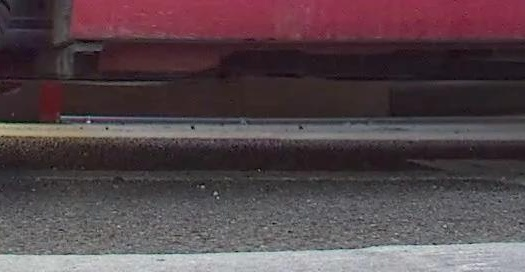
\includegraphics[width=6cm]{uncertain1.jpeg}
    %     \caption{Example ambiguous image 1}
    %     \end{minipage}
    %     \begin{minipage}[t]{0.48\textwidth}
    %     \label{uncertain2}
    %     \centering
    %     \includegraphics[width=6cm{uncertain2.jpeg}
    %     \caption{Example ambiguous image 2}
    %     \end{minipage}
    % \end{figure}
    
    \item The results we get are only based on the images of car damage. The performance is not guaranteed on other datasets.
\end{enumerate}

\subsection{Proposed Answer to the Research Question}
\begin{enumerate}
    \item 
    Q: What machine learning algorithms can help us overcome the problem of lack of labelled dataset?\\
    A: Through our research, we found the two most effective algorithms to solve this problem from different perspectives. All these algorithms were implemented in our project. The first one is active learning and the second one is semi-supervised learning.\\
    In the active learning model, it picks out the most uncertain images and sends them for retraining. Continuously, the model learns a wide variety of data distributions and the trained model will be robust. In this process, we only need to manually label fewer images because we believe that most images follow the same distribution and we only need to label some of them with unique distributions.
    \item 
    Q: What kinds of machine learning algorithms help us to correct false labeled images in real time?\\
    A: In our project, we implement continuous learning to achieve such a function. We first predict the input image, and if the predicted label is wrong, then we correct its label and feed this manually labeled image into continuous learning. In practice, we will train the continuous learning model on several images with incorrect predictions.\\
    \item 
    Q: Does the resolution affect the accuracy of the classification?\\
    A: From multiple pairs of comparisons we found that the resolution can help to improve the accuracy however the extent of the improvement is quite limited and is not comparable with the improvement brought by the augmentation operation directly on the non-enlarged dataset.\\
\end{enumerate}

\newpage

\section{Conclusion}

\subsection{Summary of the Results}
So far, we have completed our project. In the classification model, both VGG16 model and ResNet18 model perform very well. They are both applicable to our project. By comparing the active learning model with semi-supervised learning, we found that active learning performs better than semi-supervised learning on both the validation dataset and the supplemental dataset. We believe this is because the manual labeling feature in active learning helps to provide more robust labels. We prefer to use active learning models in our projects. Furthermore, we can conclude that continuous learning maintains the capability of the underlying model and also allows learning new data distributions from new images. This allows for error correction capabilities.



\subsection{Future Work}
Obviously, our project is still far from perfect. Firstly, we did not realize a universal function to find the most uncertain image for any model. We plan to add it to the website so that users can choose to upload an image themselves to predict or let the model find the most uncertain images to predict. Finding the most uncertain images is beneficial for further improving the performance.\\

Secondly, we did not add the function of training a model from scratch to the website. It is a pity not to be able to show the process of active learning with a user interface, but now only support active learning in the terminal.\\

Thirdly, the models we used were not state-of-the-art ones. For example, the SimCLR algorithm has the latest version of SimCLR v2 and Resnet is already not the best model on ImageNet \cite{ref1}.\\

Finally, a classification algorithm can not meet real-world requirements. We plan to further use Yolo or MaskRCNN to detect the damages from the images of a whole car and classify them.\\



\newpage

\section{Comments to the Group Work Experience}
To organize a group of 9 members is not easy. Everyone has his/her own schedule, forte, knowledge background. But we have the same goal: to implement a machine learning model with user interface, and all the members are willing to do their parts of jobs.\\

The strategy of our organization is to select two project managers. One controls the development processing and the other one controls the quality of output. And each group member is allocated a piece of work regarding their ability, willing and time restriction.\\

The problems in group work are mainly focused on communications, which is to convey the requirements clearly to the teammates and provide exact output to your downstream. We chose arranging point-to-point meetings to solve this problems.\\

At first we tried to use some project management tools to control the development, and using CD/CI to speed up it. However, we found it takes more time to a have every member learning such a tool than to communicate directly in the group chat, and our project is not complicated enough to use such advanced tools.\\


\newpage
\begin{thebibliography}{99}  
\bibitem{ref1}Chen, Ting, et al. "Big self-supervised models are strong semi-supervised learners." Advances in neural information processing systems 33 (2020): 22243-22255.
\bibitem{ref2}Chen, Ting, et al. "A simple framework for contrastive learning of visual representations." International conference on machine learning. PMLR, 2020.
\bibitem{ref3}Lomonaco, Vincenzo, et al. "Avalanche: an end-to-end library for continual learning." Proceedings of the IEEE/CVF Conference on Computer Vision and Pattern Recognition. 2021.
\bibitem{ref4}Blok, Pieter M., et al. "Active learning with MaskAL reduces annotation effort for training Mask R-CNN." arXiv preprint arXiv:2112.06586 (2021).
\bibitem{ref5}https://github.com/baal-org/baal.
\end{thebibliography}


\newpage
\begin{appendices}
\section{Appendix}
\begin{center}
\begin{enumerate}
    \item Training process of supervised learning of ResNet and VGG
        \begin{figure}[h]
        \centering
        \subfigure[VGG Best]{
        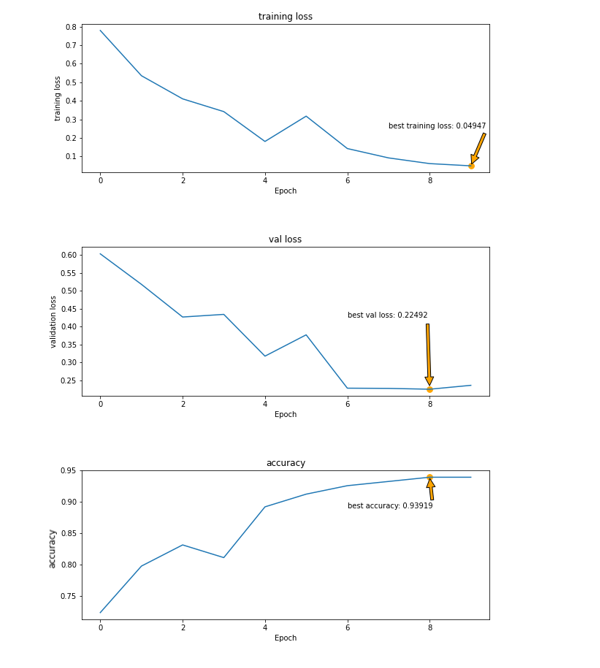
\includegraphics[scale=0.65]{VGG16best.png}}
        \subfigure[ResNet Best]{
        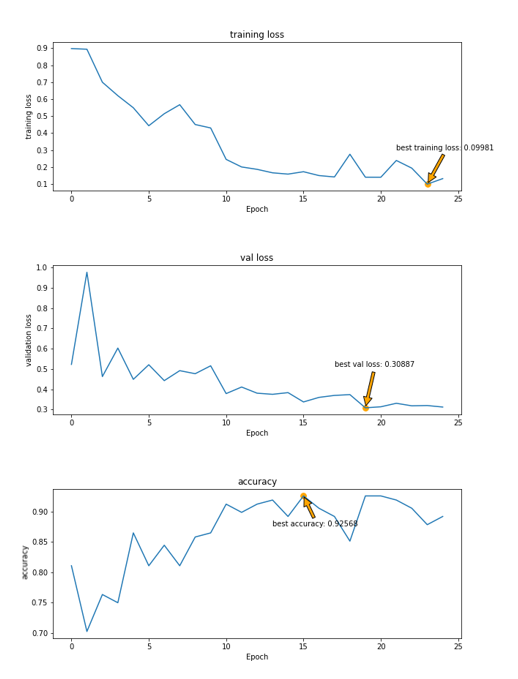
\includegraphics[scale=0.65]{ResNetbest.png}}
        \end{figure}
    \item Training process of active learning
        \begin{figure}[H]
        \centering
        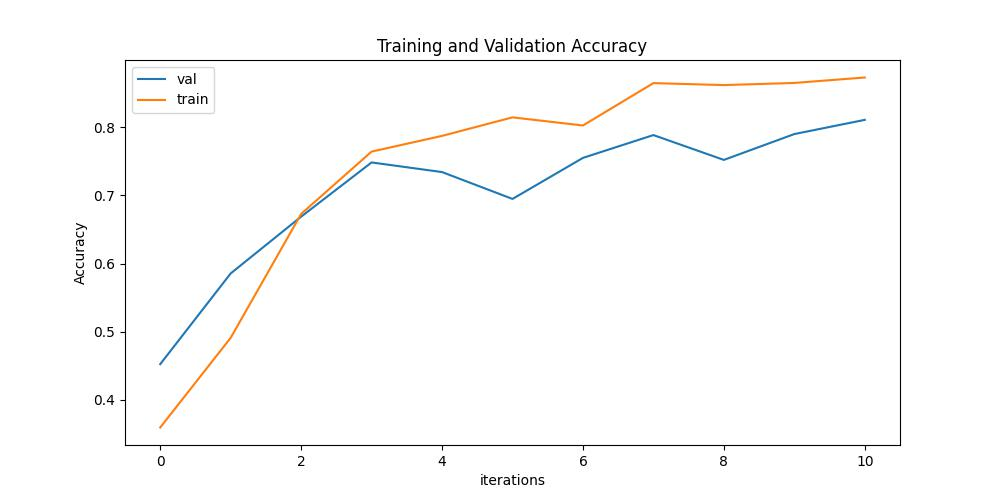
\includegraphics[scale=0.4]{TrainingAndValidationAccuracy.png}
        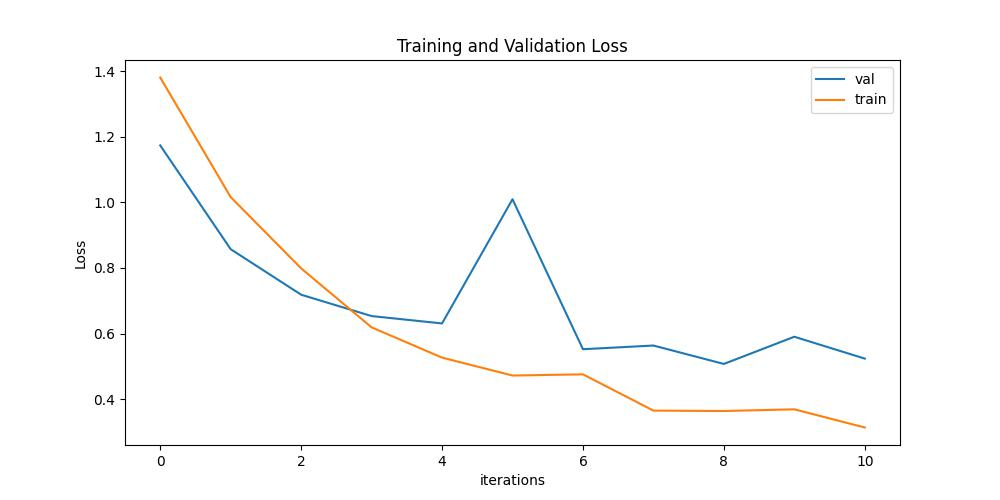
\includegraphics[scale=0.4]{TrainingAndValidationLoss.png}
        \caption{Training and validation accuracy and loss}
        \end{figure}
    \item Training process of continual learning with LWF
        \begin{figure}[H]
        \centering
        \subfigure[Accuracy]{
        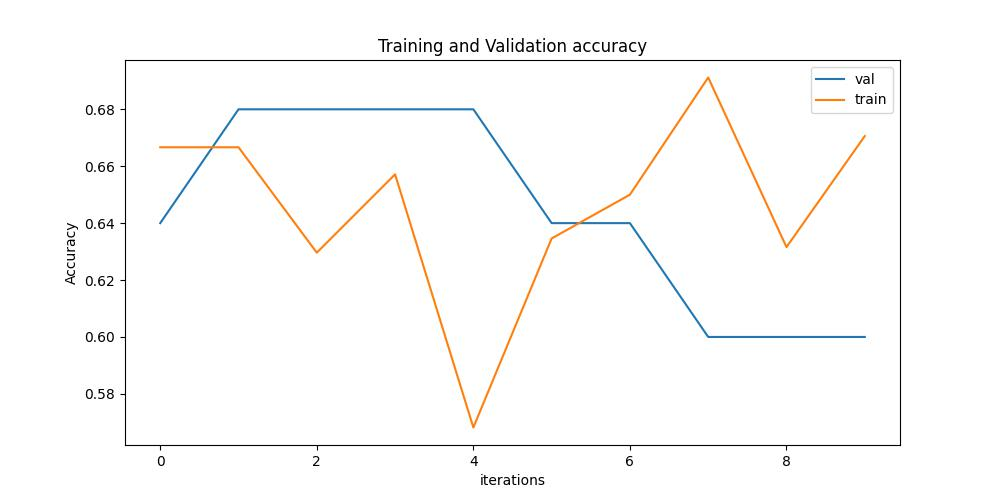
\includegraphics[scale=0.27]{conV1.png}}
        \subfigure[Loss]{
        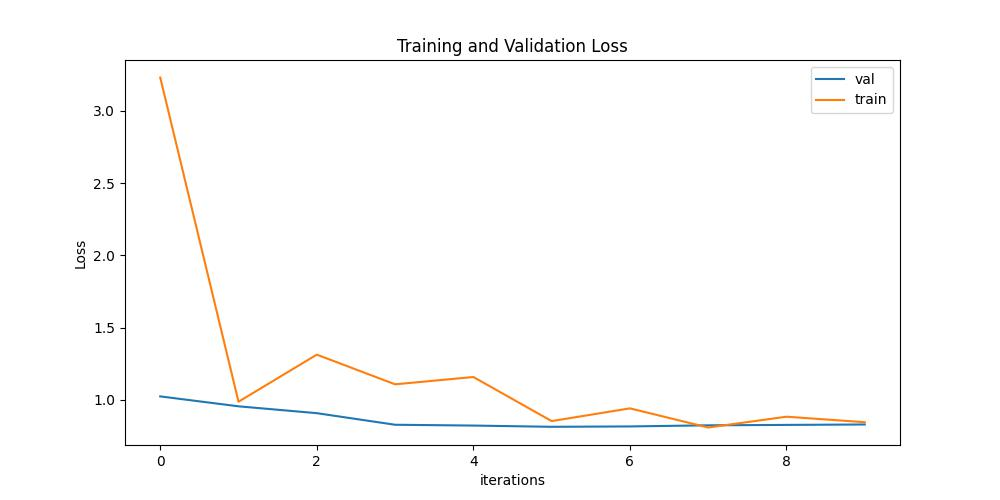
\includegraphics[scale=0.27]{conV2.png}}
        \caption{VGG16's Training and validation accuracy and loss}
        \end{figure}

        \begin{figure}[H]
        \centering
        \subfigure[Accuracy]{
        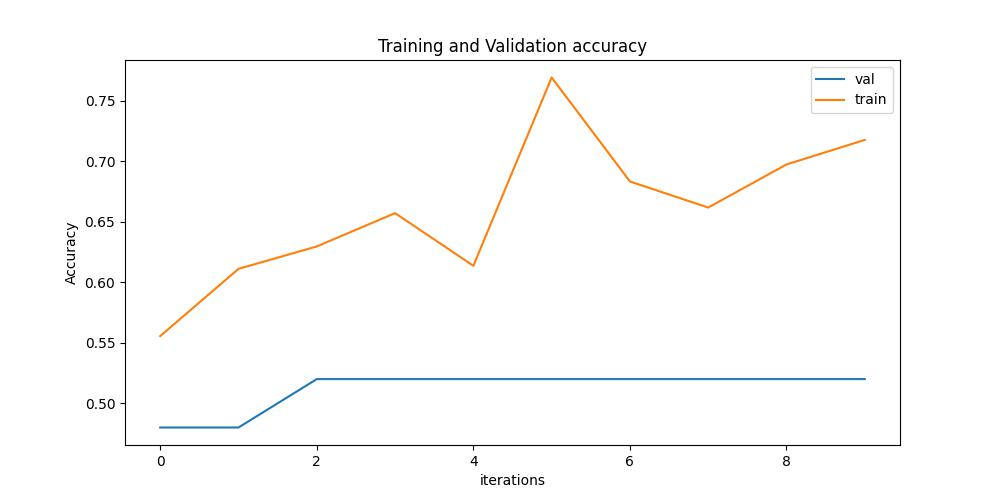
\includegraphics[scale=0.27]{conRe1.png}}
        \subfigure[Loss]{
        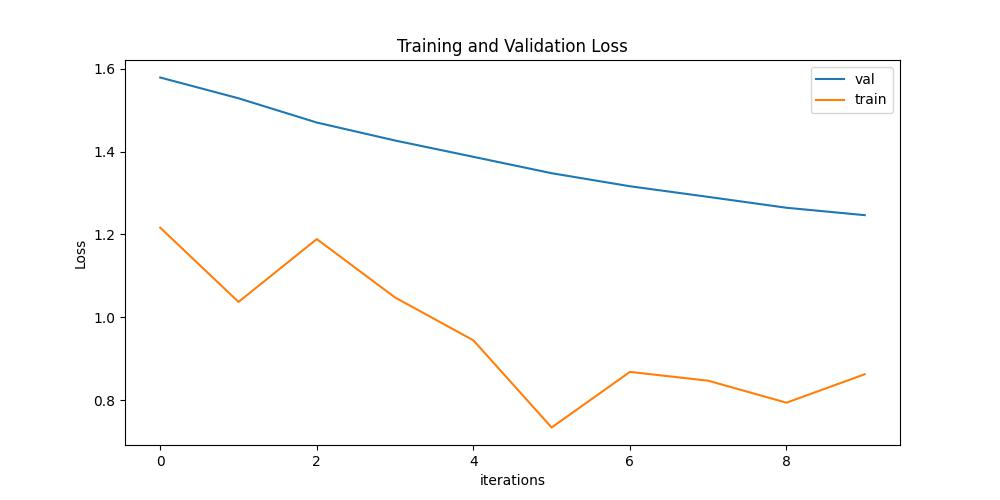
\includegraphics[scale=0.27]{conRe2.png}}
        \caption{ResNet18's Training and validation accuracy and loss}
        \end{figure}
    \item Training process of continual learning with LWF
        \begin{figure}[H]
        \centering
        \subfigure[Accuracy]{
        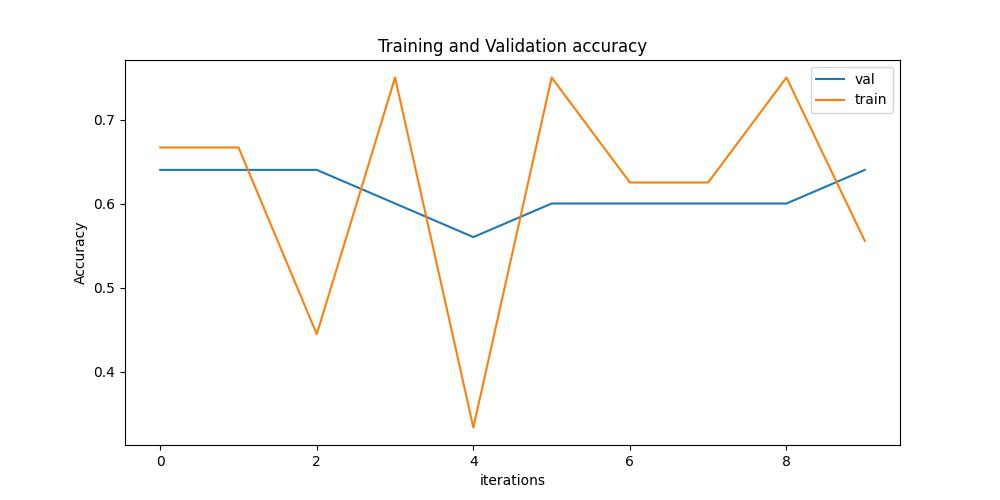
\includegraphics[scale=0.27]{conV11.png}}
        \subfigure[Loss]{
        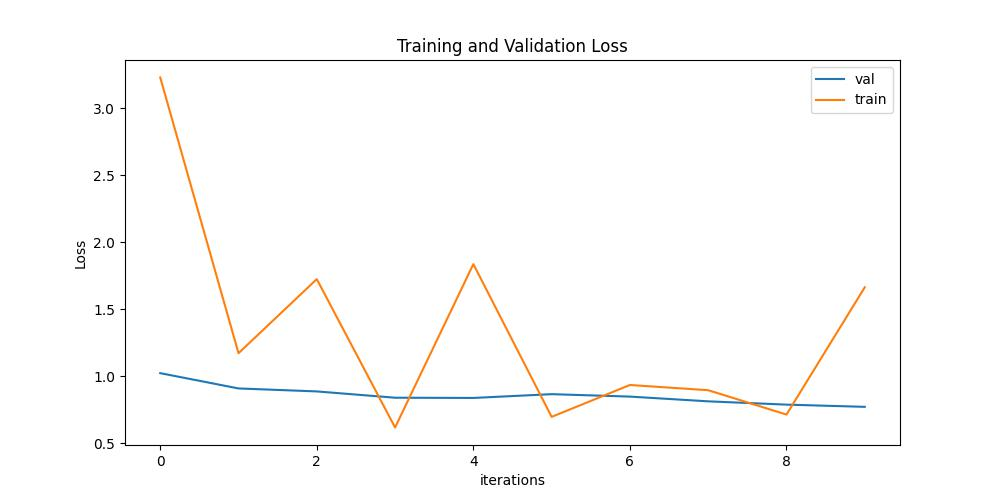
\includegraphics[scale=0.27]{conV22.png}}
        \caption{accuracy and loss of LWF stragety of VGG16}
        \end{figure}
        \begin{figure}[H]
        \centering
        \subfigure[Accuracy]{
        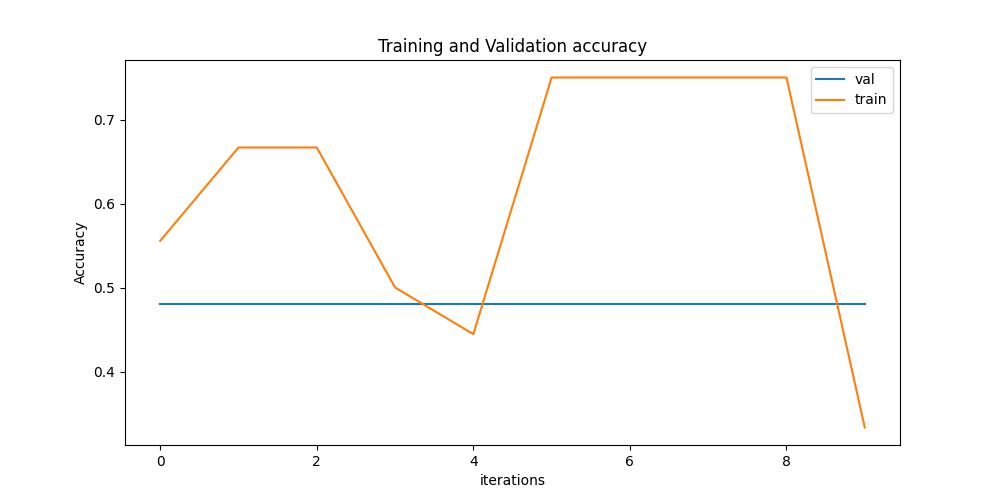
\includegraphics[scale=0.27]{conRe11.png}}
        \subfigure[Loss]{
        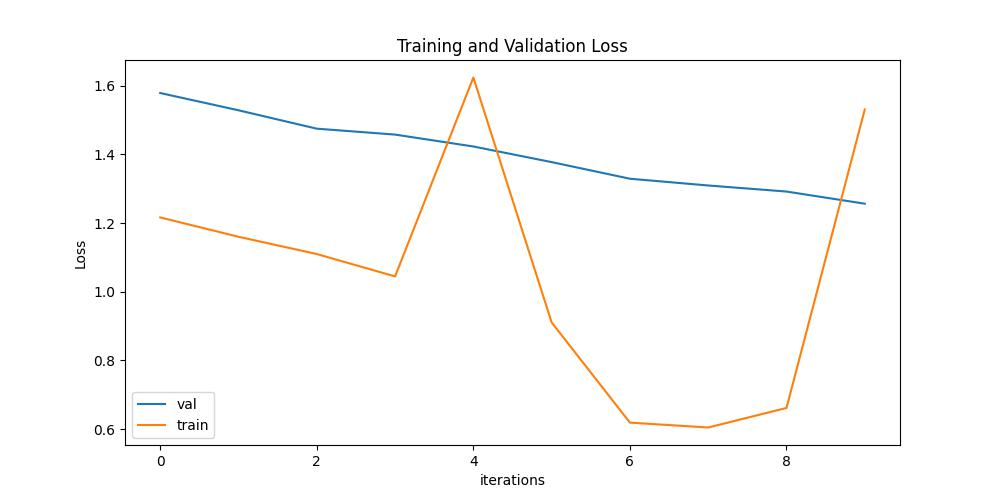
\includegraphics[scale=0.27]{conRe22.png}}
        \caption{ResNet18's Training and validation accuracy and loss}
        \end{figure}    

\end{enumerate}

\end{center} 
\end{appendices}

\end{document}
